\documentclass{article}
\usepackage[utf8]{inputenc}
\usepackage{hyperref}

% TEMPLATE COMMENTS FORMATTING
\usepackage{amsmath,amssymb}
\usepackage{ifthen}
\usepackage{subcaption}
\usepackage[dvipsnames]{xcolor}
\usepackage[most]{tcolorbox}
\usepackage{soul}
\newboolean{showcomments}
\setboolean{showcomments}{true}
\ifthenelse{\boolean{showcomments}}
{\newcommand{\nb}[2] {
\fcolorbox{yellow}{yellow!20}{\bfseries\sffamily\scriptsize#1:}
{\sf\small$\blacktriangleright$\textit{#2}$\blacktriangleleft$}
}
}
{\newcommand{\nb}[2]{}
}
\newcommand\templateInstruction[1]{
% \nb{Template}{
\hl{#1}
% }
}
\newcommand\templateExample[1]{
\nb{Example}{
\hl{#1}
}
}
%



\title{IMA Project 1: God Classes}
\author{{Navdeep Singh Bedi} }
\date{\today}

\begin{document}

\setcounter{section}{-1}

\maketitle

% The following shows a minimal submission report for project 1. If you choose to use this template, replace all template instructions (the yellow bits) with your own values.
% In addition, for any section, if \textbf{and only if} anything was unclear or warnings were raised by the code, and you had to take assumptions about the correct implementation (e.g., about details of a metric), describe your assumptions in one or two sentences.

% You may - at your own risk - also choose not to use this template. As long as your submission is a latex-generated, English PDF containing all expected info, you'll be fine.

\textbf{God class} is the classe in OOP which violate the single responsibility principle i.e, it provide
too many functionalities inside the same class and thus make the class higly unfocused.

The main goal of the project is to use clustering to to support automated refactoring of God classes. 

The project goes as follows: 

\begin{enumerate}
    \item We start with identifying God classes inside the given \textit{xerces2-j-src} repository.
    \item Next we extract the feature vectors of the classes based on the class methods and attributes and field methods and attributes.
    \item Then we clustering algorithms such as k-means and Agglomerative to cluster the God classes based on the feature vectors.
    \item Finally we measure the quality of the God class partitions using Precision and Recall scores.
\end{enumerate}

\section{Code Repository}

The code and result files, part of this submission, can be found at:

\begin{center}
    Repo: {https://github.com/infoMA2023/project-01-god-classes-navdeeps350.git} \\
    Commit: e9067a5
\end{center}

\section{Data Pre-Processing}
The data preprocessing takes place in two parts:
\begin{enumerate}
    \item Identification of God classes.
    \item Extraction of feature vectors from the God classes.
\end{enumerate}
The steps for the preprocessing are given below.
\subsection{God Classes}
To identify the God classes we parse the source code in given repository using \textit{javalang} library of Python and 
count the number of methods in each class without counting the methods in the 
subclass of the class. This gives the number of methods present in each class of the repository,
and then with the help of the given eq.\ref{eq:1}:
\begin{equation}
    God(C) \iff | M(C) | > \mu(M) + 6\sigma(M)
    \label{eq:1}
\end{equation}
\begin{table}[]
    \centering
    \begin{tabular}{lc}
        \hline
        \textbf{Class Name} &\textbf{\# Methods} \\
        \hline\hline
        {XSDHandler} & {118}\\
        {DTDGrammar} & {101}\\
        {XIncludeHandler} & {116}\\
        {CoreDocumentImpl} & {125}\\
        \hline
    \end{tabular}
    \caption{Identified God Classes}
    \label{tab:god_classes}
\end{table}
where M(C) is the set of methods in class C; M is the set of all methods across all classes
The god classes I identified, and their corresponding number of methods can be found in Table \ref{tab:god_classes}.

The code for this step can be found in \textit{find\_god\_classes.py} file.
To run the code, the user needs to provide the path (\textit{resources/xerces2-j-src}, in this case) to the repository as an argument to the script.
The output of the script is a file named \textit{god\_classes.csv} in the \textit{results\_csv} folder.
\subsection{Feature Vectors}
In the second step, we extract the feature vectors of the extracted God classes in the previous step. This is done as follows:
\begin{enumerate}
    \item First, we select only those class matching the input file name, to skip inner classes.
    \item Then for this class in each of the file extracted, we find the field and 
    the method names present in the class and also the fields and methods accessed in the particular method in that class.
    Doing this we only take the methods and fields present in the God class.
    \item We populate the nested dictionary with the method name as a key and the corresponding valid field and method names present in that method with their counter (inner dictionary) as the value. 
    \item Then we create a dataframe with all the methods present in the class as rows and all the valid fields and methods (used atleast once) in class as columns.
    \item Finally we populate the data frame accordingly with the help of dictionary and replace the counter value with 1's and 0's if the corresponding valid field and method is accessed in the given method or not.
\end{enumerate}

Table \ref{tab:feat_vec} shows aggregate numbers regarding the extracted feature vectors for the god classes.
\begin{table}[]
    \centering
    \begin{tabular}{lcc}
        \hline
        \textbf{Class Name} &\textbf{\# Feature Vectors} & \textbf{\# Attributes*}\\
        \hline\hline
        {XSDHandler} & {106} & {194}\\
        {DTDGrammar} & {91} & {102}\\
        {XIncludeHandler} & {108} & {183}\\
        {CoreDocumentImpl} & {117} & {66}\\
        \hline
    \end{tabular}
    \caption{Feature vector summary (*= used at least once)}
    \label{tab:feat_vec}
\end{table}

The code for this step can be found in \textit{extract\_feature\_vectors.py} file.
The corresponding output file is named \textit{filepath.csv} (different for different file paths) in the \textit{results\_csv} folder.

\section{Clustering}
\label{sec:clustering}

\subsection{Algorithm Configurations}
% \templateInstruction{Report/comment the algorithm configurations (distance function, linkage rule, etc.). You may do so in any form you feel suited, but a short paragraph of text is probably sufficient.}
Two algorithms were used for clustering: Agglomerative and k-means. For Agglomerative clustering, the distance function used was Euclidean. In both the casses the feature vectors file created in the previous step was used as an input and the 
number of clusters was asked from the user as input. The code for this step can be found in \textit{k\_means.py} and \textit{hierarchical.py} file.
And the results of the clustering can be found in the \textit{results\_csv} folder and the nomenclature of the different results file is explained in the code.
Both the files can be run by providing the path to the feature vectors file created in the Part-02 of this project present in the \textit{results\_csv} folder and the number of clusters as an argument to the script.

\subsection{Testing Various k \& Silhouette Scores}
The next step is to test the clustering algorithms for various values of k. The results of the clustering are evaluated using the silhouette score.
The silhouette score is a measure of how similar an object is to its cluster compared to other clusters. The silhouette score ranges from -1 to 1, where a high value indicates that the object is well matched to its own cluster and poorly matched to neighboring clusters.
The code for this step can be found in \textit{silhouette.py} file.
To run the code, the user either can provide just the path to the feature vectors file as an argument to the script or can provide both the path to the feature vectors file and the path to the corresponding cluster file created in the last part as an argument to the script.
In the first case, the script will run the clustering for the values of k from 2 to 59 and will calculate the corresponding silhouette score for each value of k and for both the algorithms. In the second case, the script will calculate the silhouette score for the given cluster file.

The output of the script is a file named \textit{filename\_silhouette\_scores.csv} in the \textit{results\_csv} folder in the first case and in the second case it is printed on the console.

The summarization of silhouette scores for the optimal number of clusters is as follows:
\begin{enumerate}
    \item We found out that for the file \textit{CoreDocumentImpl.csv} the optimal number of clusters in case of k-means increases with the increase in the number of clusters, so the maximum is achieved at k = 59, while in case of agglomerative clustering the optimal number of clusters is achieved at k = 45. The silhouette scores for the optimal number of clusters can be found in the \textit{CoreDocumentImpl\_silhouette\_scores.csv} file in the \textit{results\_csv} folder.
    \item For the file \textit{DTDGrammar.csv} the optimal number of clusters in case of both the clustering algorithms is achieved at k = 58. The silhouette scores for the optimal number of clusters can be found in the \textit{DTDGrammar\_silhouette\_scores.csv} file in the \textit{results\_csv} folder.
    \item For the file \textit{XSDIncludeHandler.csv} the optimal number of clusters in case of k-means is achieved in the beginning at k = 4, while in case of agglomerative clustering the optimal number of clusters is achieved at k = 2. The silhouette scores for the optimal number of clusters can be found in the \textit{XSDIncludeHandler\_silhouette\_scores.csv} file in the \textit{results\_csv} folder.
    \item For the file \textit{XSDHandler.csv} the optimal number of clusters in case of both the clustering algorithms are achived at k = 2. The silhouette scores for the optimal number of clusters can be found in the \textit{XSDHandler\_silhouette\_scores.csv} file in the \textit{results\_csv} folder.
\end{enumerate}
The corresponding graphs for the silhouette scores for the optimal number of clusters can be found in the \textit{results\_csv} folder.
\begin{figure}
	\centering
	\begin{minipage}{0.45\linewidth}
	     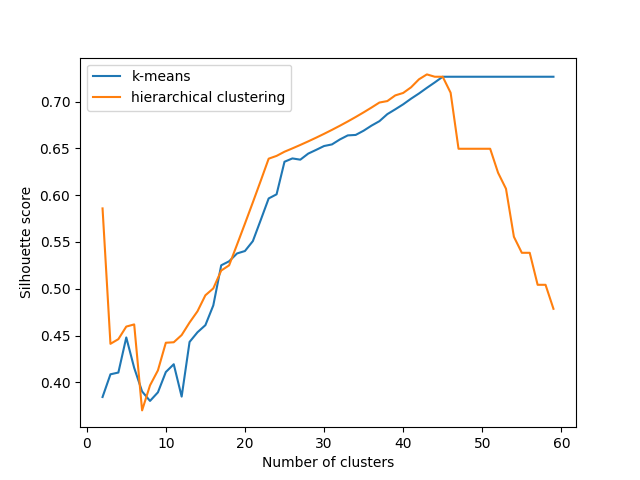
\includegraphics[width=\linewidth]{CoreDocumentImpl_silhouette_scores.png}
	      \subcaption{CoreDocumentImpl}
	      \label{fig:subfig1}
	\end{minipage}
	\begin{minipage}{0.45\linewidth}
	    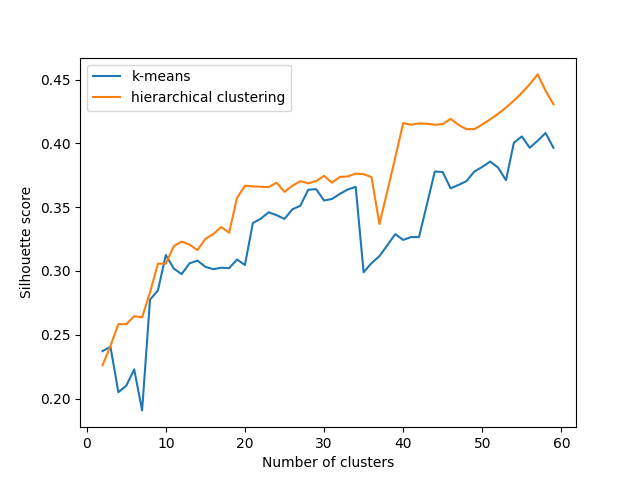
\includegraphics[width=\linewidth]{DTDGrammar_silhouette_scores.png}
	    \subcaption{DTDGrammar}
	    \label{fig:subfig2}
        \end{minipage} \\	
	\begin{minipage}{0.45\linewidth}
	    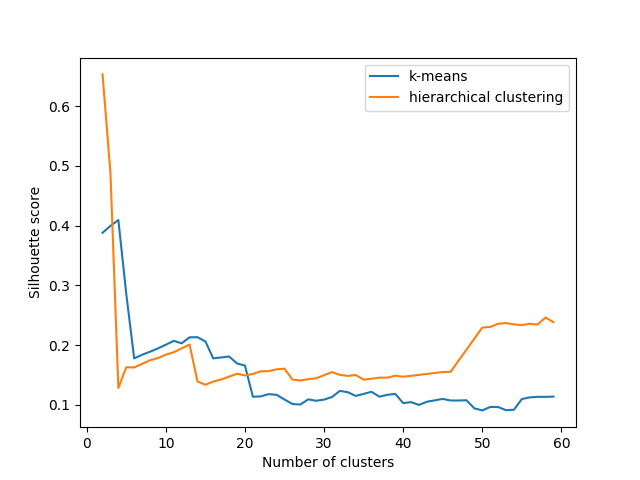
\includegraphics[width=\linewidth]{XIncludeHandler_silhouette_scores.png}
	    \subcaption{XIncludeHandler}
	\label{fig:subfig3}
         \end{minipage}
         \begin{minipage}{0.45\linewidth}
	    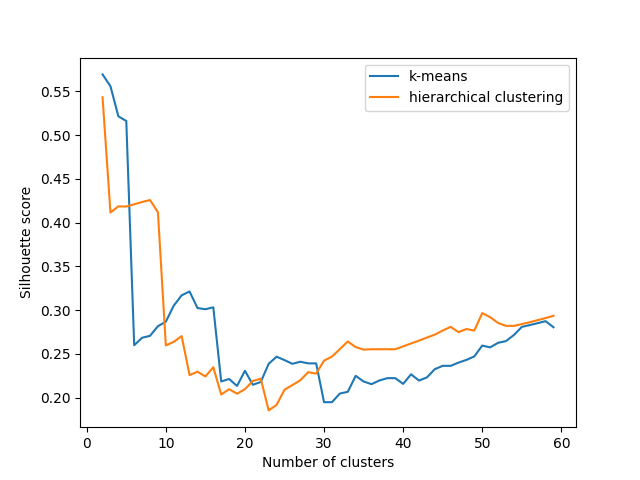
\includegraphics[width=\linewidth]{XSDHandler_silhouette_scores.png}
	    \subcaption{XSDHandler}
	\label{fig:subfig4}
         \end{minipage}
\caption{Silhouette scores for the clusters from k = 2 to 59.}
\label{fig:fig1}
\end{figure}
The corresponding graphs for the silhouette scores for the clusters from k = 2 to 59, for the God Classes are shown in the fig.\ref{fig:fig1}
% (1) Report data about the clusters produced by the two algorithms at various k
% (\#clusters, size of clusters, silhouette scores). You may use any suitable format (table, graph, ...).

% (2) Briefly comment your results. What is the best configuration, and why? Anything else you observed?}


\section{Evaluation}
The evaluation of the models is done in two steps:
\begin{enumerate}
    \item Defining the ground truth.
    \item Computing the precision, recall scores and F1 scores for the optimal configurations found discussed below.
\end{enumerate}
\subsection{Ground Truth}
% I computed the ground truth using the command \templateInstruction{...}. The generated files are checked into the repository with the names \templateInstruction{...}.
As we are not the writers of the \textit{xerces2-j-src} repository, we do not have the ground truth for the God classes in the repository. So, we created the ground truth by manually according to the keywords given in the Part-04 of the project slides. The keywords can be found in the \textit{keywords.txt} file.
To define the ground truth labels for each method of the God classes, we used the keywords present in the \textit{keywords.txt} file. If any of the keywords is present in the method name, then the method is labeled as according to that keyword and if multiple keywords are present in the method name then the first keyword determines the cluster label for that method. 
If none of the keyword is present in the method name, then the method is labeled as in '\textit{other}' cluster. 
The cluster labeles are then converted into numerical values for the evaluation of the clustering algorithms.

Though the ground truth is not perfect. The drawback of the ground truth is that it is based on the keywords present in the method names and the keywords are not exhaustive, so the ground truth may not be perfect.
And in the case of the multiple ground truth labels for a single method, we have taken the first keyword as the cluster label for that method, which may not be the correct way to label the method.
Still, it is a good approximation of the actual ground truth.


% \templateInstruction{Comment briefly on the strengths \& weaknesses of our ground truth.}

\subsection{Precision and Recall}
For calculating the precision and recall scores, we used the ground truth labels and the calculated cluster labels obtained from the clustering algorithms. 
The number of clusters in the clustering algorithms is set to the number of clusters in the ground truth labels. The code for this step can be found in the \textit{prec\_recall.py} file.
To run the code, the user needs to provide the path to the ground truth file and the path to the cluster file as an argument to the script.
We used the number of cluster labels in the ground truth instead of the optimal number of clusters give by the silhouette score because of in some of the God classes the silhouette score increases with the number of clusters and it wouldn't make sense to use for example,
5 clusters for the ground truth and 59 clusters for the clustering algorithms.
\begin{table}[]
    \centering
    \begin{tabular}{lcccc}
        \hline
        \textbf{Class Name} &\multicolumn{2}{c}{\textbf{Agglomerative}} & \multicolumn{2}{c}{\textbf{K-Means}} \\
        \hline
         &Prec. & Recall & Prec. & Recall \\
        \hline\hline
        {CoreDocumentImpl} & {0.47} & {0.52}& {0.45}& {0.69}\\
       {DTDGrammar} & {0.54} & {0.47}& {0.54}& {0.35}\\
        {XIncludeHandler} & {0.66} & {0.46}& {0.67}& {0.77}\\
        {XSDHandler} & {0.35} & {0.72}& {0.36}& {0.89}\\
        \hline
    \end{tabular}
    \caption{Evaluation Summary}
    \label{tab:eval}
\end{table}

Precision and Recall, for the configurations found in Section \ref{sec:clustering}, are reported in Table \ref{tab:eval}.


\subsection{Practical Usefulness}
% \templateInstruction{Discuss the practical usefulness of the obtained code refactoring assistant in a realistic setting (1 paragraph).}
The practical usefulness of the obtained code refactoring assistant in a realistic setting is that it can be used to identify the God classes in the repository and then can be used to refactor the code by breaking the God classes into smaller classes with single responsibility. 
This will make the code more maintainable and understandable. 
\end{document}
